
%% bare_conf.tex
%% V1.3
%% 2007/01/11
%% by Michael Shell
%% See:
%% http://www.michaelshell.org/
%% for current contact information.
%%
%% This is a skeleton file demonstrating the use of IEEEtran.cls
%% (requires IEEEtran.cls version 1.7 or later) with an IEEE conference paper.
%%
%% Support sites:
%% http://www.michaelshell.org/tex/ieeetran/
%% http://www.ctan.org/tex-archive/macros/latex/contrib/IEEEtran/
%% and
%% http://www.ieee.org/

%%*************************************************************************
%% Legal Notice:
%% This code is offered as-is without any warranty either expressed or
%% implied; without even the implied warranty of MERCHANTABILITY or
%% FITNESS FOR A PARTICULAR PURPOSE! 
%% User assumes all risk.
%% In no event shall IEEE or any contributor to this code be liable for
%% any damages or losses, including, but not limited to, incidental,
%% consequential, or any other damages, resulting from the use or misuse
%% of any information contained here.
%%
%% All comments are the opinions of their respective authors and are not
%% necessarily endorsed by the IEEE.
%%
%% This work is distributed under the LaTeX Project Public License (LPPL)
%% ( http://www.latex-project.org/ ) version 1.3, and may be freely used,
%% distributed and modified. A copy of the LPPL, version 1.3, is included
%% in the base LaTeX documentation of all distributions of LaTeX released
%% 2003/12/01 or later.
%% Retain all contribution notices and credits.
%% ** Modified files should be clearly indicated as such, including  **
%% ** renaming them and changing author support contact information. **
%%
%% File list of work: IEEEtran.cls, IEEEtran_HOWTO.pdf, bare_adv.tex,
%%                    bare_conf.tex, bare_jrnl.tex, bare_jrnl_compsoc.tex
%%*************************************************************************

% *** Authors should verify (and, if needed, correct) their LaTeX system  ***
% *** with the testflow diagnostic prior to trusting their LaTeX platform ***
% *** with production work. IEEE's font choices can trigger bugs that do  ***
% *** not appear when using other class files.                            ***
% The testflow support page is at:
% http://www.michaelshell.org/tex/testflow/



% Note that the a4paper option is mainly intended so that authors in
% countries using A4 can easily print to A4 and see how their papers will
% look in print - the typesetting of the document will not typically be
% affected with changes in paper size (but the bottom and side margins will).
% Use the testflow package mentioned above to verify correct handling of
% both paper sizes by the user's LaTeX system.
%
% Also note that the "draftcls" or "draftclsnofoot", not "draft", option
% should be used if it is desired that the figures are to be displayed in
% draft mode.
%
\documentclass[conference]{IEEEtran}
% Add the compsoc option for Computer Society conferences.
%
% If IEEEtran.cls has not been installed into the LaTeX system files,
% manually specify the path to it like:
%\documentclass[conference]{../sty/IEEEtran}





% Some very useful LaTeX packages include:
% (uncomment the ones you want to load)


% *** MISC UTILITY PACKAGES ***
%
%\usepackage{ifpdf}
% Heiko Oberdiek's ifpdf.sty is very useful if you need conditional
% compilation based on whether the output is pdf or dvi.
% usage:
% \ifpdf
%   % pdf code
% \else
%   % dvi code
% \fi
% The latest version of ifpdf.sty can be obtained from:
% http://www.ctan.org/tex-archive/macros/latex/contrib/oberdiek/
% Also, note that IEEEtran.cls V1.7 and later provides a builtin
% \ifCLASSINFOpdf conditional that works the same way.
% When switching from latex to pdflatex and vice-versa, the compiler may
% have to be run twice to clear warning/error messages.






% *** CITATION PACKAGES ***
%
\usepackage{cite}
% cite.sty was written by Donald Arseneau
% V1.6 and later of IEEEtran pre-defines the format of the cite.sty package
% \cite{} output to follow that of IEEE. Loading the cite package will
% result in citation numbers being automatically sorted and properly
% "compressed/ranged". e.g., [1], [9], [2], [7], [5], [6] without using
% cite.sty will become [1], [2], [5]--[7], [9] using cite.sty. cite.sty's
% \cite will automatically add leading space, if needed. Use cite.sty's
% noadjust option (cite.sty V3.8 and later) if you want to turn this off.
% cite.sty is already installed on most LaTeX systems. Be sure and use
% version 4.0 (2003-05-27) and later if using hyperref.sty. cite.sty does
% not currently provide for hyperlinked citations.
% The latest version can be obtained at:
% http://www.ctan.org/tex-archive/macros/latex/contrib/cite/
% The documentation is contained in the cite.sty file itself.






% *** GRAPHICS RELATED PACKAGES ***
%
\ifCLASSINFOpdf
\usepackage[pdftex]{graphicx}
  % declare the path(s) where your graphic files are
  % \graphicspath{{../pdf/}{../jpeg/}}
  % and their extensions so you won't have to specify these with
  % every instance of \includegraphics
  % \DeclareGraphicsExtensions{.pdf,.jpeg,.png}
\else
  % or other class option (dvipsone, dvipdf, if not using dvips). graphicx
  % will default to the driver specified in the system graphics.cfg if no
  % driver is specified.
  % \usepackage[dvips]{graphicx}
  % declare the path(s) where your graphic files are
  % \graphicspath{{../eps/}}
  % and their extensions so you won't have to specify these with
  % every instance of \includegraphics
  % \DeclareGraphicsExtensions{.eps}
\fi
% graphicx was written by David Carlisle and Sebastian Rahtz. It is
% required if you want graphics, photos, etc. graphicx.sty is already
% installed on most LaTeX systems. The latest version and documentation can
% be obtained at: 
% http://www.ctan.org/tex-archive/macros/latex/required/graphics/
% Another good source of documentation is "Using Imported Graphics in
% LaTeX2e" by Keith Reckdahl which can be found as epslatex.ps or
% epslatex.pdf at: http://www.ctan.org/tex-archive/info/
%
% latex, and pdflatex in dvi mode, support graphics in encapsulated
% postscript (.eps) format. pdflatex in pdf mode supports graphics
% in .pdf, .jpeg, .png and .mps (metapost) formats. Users should ensure
% that all non-photo figures use a vector format (.eps, .pdf, .mps) and
% not a bitmapped formats (.jpeg, .png). IEEE frowns on bitmapped formats
% which can result in "jaggedy"/blurry rendering of lines and letters as
% well as large increases in file sizes.
%
% You can find documentation about the pdfTeX application at:
% http://www.tug.org/applications/pdftex





% *** MATH PACKAGES ***
%
%\usepackage[cmex10]{amsmath}
% A popular package from the American Mathematical Society that provides
% many useful and powerful commands for dealing with mathematics. If using
% it, be sure to load this package with the cmex10 option to ensure that
% only type 1 fonts will utilized at all point sizes. Without this option,
% it is possible that some math symbols, particularly those within
% footnotes, will be rendered in bitmap form which will result in a
% document that can not be IEEE Xplore compliant!
%
% Also, note that the amsmath package sets \interdisplaylinepenalty to 10000
% thus preventing page breaks from occurring within multiline equations. Use:
%\interdisplaylinepenalty=2500
% after loading amsmath to restore such page breaks as IEEEtran.cls normally
% does. amsmath.sty is already installed on most LaTeX systems. The latest
% version and documentation can be obtained at:
% http://www.ctan.org/tex-archive/macros/latex/required/amslatex/math/





% *** SPECIALIZED LIST PACKAGES ***
%
\usepackage{algorithmic}
% algorithmic.sty was written by Peter Williams and Rogerio Brito.
% This package provides an algorithmic environment fo describing algorithms.
% You can use the algorithmic environment in-text or within a figure
% environment to provide for a floating algorithm. Do NOT use the algorithm
% floating environment provided by algorithm.sty (by the same authors) or
% algorithm2e.sty (by Christophe Fiorio) as IEEE does not use dedicated
% algorithm float types and packages that provide these will not provide
% correct IEEE style captions. The latest version and documentation of
% algorithmic.sty can be obtained at:
% http://www.ctan.org/tex-archive/macros/latex/contrib/algorithms/
% There is also a support site at:
% http://algorithms.berlios.de/index.html
% Also of interest may be the (relatively newer and more customizable)
% algorithmicx.sty package by Szasz Janos:
% http://www.ctan.org/tex-archive/macros/latex/contrib/algorithmicx/




% *** ALIGNMENT PACKAGES ***
%
%\usepackage{array}
% Frank Mittelbach's and David Carlisle's array.sty patches and improves
% the standard LaTeX2e array and tabular environments to provide better
% appearance and additional user controls. As the default LaTeX2e table
% generation code is lacking to the point of almost being broken with
% respect to the quality of the end results, all users are strongly
% advised to use an enhanced (at the very least that provided by array.sty)
% set of table tools. array.sty is already installed on most systems. The
% latest version and documentation can be obtained at:
% http://www.ctan.org/tex-archive/macros/latex/required/tools/


%\usepackage{mdwmath}
%\usepackage{mdwtab}
% Also highly recommended is Mark Wooding's extremely powerful MDW tools,
% especially mdwmath.sty and mdwtab.sty which are used to format equations
% and tables, respectively. The MDWtools set is already installed on most
% LaTeX systems. The lastest version and documentation is available at:
% http://www.ctan.org/tex-archive/macros/latex/contrib/mdwtools/


% IEEEtran contains the IEEEeqnarray family of commands that can be used to
% generate multiline equations as well as matrices, tables, etc., of high
% quality.


%\usepackage{eqparbox}
% Also of notable interest is Scott Pakin's eqparbox package for creating
% (automatically sized) equal width boxes - aka "natural width parboxes".
% Available at:
% http://www.ctan.org/tex-archive/macros/latex/contrib/eqparbox/





% *** SUBFIGURE PACKAGES ***
%\usepackage[tight,footnotesize]{subfigure}
% subfigure.sty was written by Steven Douglas Cochran. This package makes it
% easy to put subfigures in your figures. e.g., "Figure 1a and 1b". For IEEE
% work, it is a good idea to load it with the tight package option to reduce
% the amount of white space around the subfigures. subfigure.sty is already
% installed on most LaTeX systems. The latest version and documentation can
% be obtained at:
% http://www.ctan.org/tex-archive/obsolete/macros/latex/contrib/subfigure/
% subfigure.sty has been superceeded by subfig.sty.



%\usepackage[caption=false]{caption}
%\usepackage[font=footnotesize]{subfig}
% subfig.sty, also written by Steven Douglas Cochran, is the modern
% replacement for subfigure.sty. However, subfig.sty requires and
% automatically loads Axel Sommerfeldt's caption.sty which will override
% IEEEtran.cls handling of captions and this will result in nonIEEE style
% figure/table captions. To prevent this problem, be sure and preload
% caption.sty with its "caption=false" package option. This is will preserve
% IEEEtran.cls handing of captions. Version 1.3 (2005/06/28) and later 
% (recommended due to many improvements over 1.2) of subfig.sty supports
% the caption=false option directly:
%\usepackage[caption=false,font=footnotesize]{subfig}
%
% The latest version and documentation can be obtained at:
% http://www.ctan.org/tex-archive/macros/latex/contrib/subfig/
% The latest version and documentation of caption.sty can be obtained at:
% http://www.ctan.org/tex-archive/macros/latex/contrib/caption/




% *** FLOAT PACKAGES ***
%
%\usepackage{fixltx2e}
% fixltx2e, the successor to the earlier fix2col.sty, was written by
% Frank Mittelbach and David Carlisle. This package corrects a few problems
% in the LaTeX2e kernel, the most notable of which is that in current
% LaTeX2e releases, the ordering of single and double column floats is not
% guaranteed to be preserved. Thus, an unpatched LaTeX2e can allow a
% single column figure to be placed prior to an earlier double column
% figure. The latest version and documentation can be found at:
% http://www.ctan.org/tex-archive/macros/latex/base/



%\usepackage{stfloats}
% stfloats.sty was written by Sigitas Tolusis. This package gives LaTeX2e
% the ability to do double column floats at the bottom of the page as well
% as the top. (e.g., "\begin{figure*}[!b]" is not normally possible in
% LaTeX2e). It also provides a command:
%\fnbelowfloat
% to enable the placement of footnotes below bottom floats (the standard
% LaTeX2e kernel puts them above bottom floats). This is an invasive package
% which rewrites many portions of the LaTeX2e float routines. It may not work
% with other packages that modify the LaTeX2e float routines. The latest
% version and documentation can be obtained at:
% http://www.ctan.org/tex-archive/macros/latex/contrib/sttools/
% Documentation is contained in the stfloats.sty comments as well as in the
% presfull.pdf file. Do not use the stfloats baselinefloat ability as IEEE
% does not allow \baselineskip to stretch. Authors submitting work to the
% IEEE should note that IEEE rarely uses double column equations and
% that authors should try to avoid such use. Do not be tempted to use the
% cuted.sty or midfloat.sty packages (also by Sigitas Tolusis) as IEEE does
% not format its papers in such ways.





% *** PDF, URL AND HYPERLINK PACKAGES ***
%
\usepackage{url}
% url.sty was written by Donald Arseneau. It provides better support for
% handling and breaking URLs. url.sty is already installed on most LaTeX
% systems. The latest version can be obtained at:
% http://www.ctan.org/tex-archive/macros/latex/contrib/misc/
% Read the url.sty source comments for usage information. Basically,
% \url{my_url_here}.





% *** Do not adjust lengths that control margins, column widths, etc. ***
% *** Do not use packages that alter fonts (such as pslatex).         ***
% There should be no need to do such things with IEEEtran.cls V1.6 and later.
% (Unless specifically asked to do so by the journal or conference you plan
% to submit to, of course. )


% correct bad hyphenation here
\hyphenation{op-tical net-works semi-conduc-tor}

\begin{document}
%
% paper title
% can use linebreaks \\ within to get better formatting as desired
\title{A Rent/Self-execute Model for Cloud Providers}


% author names and affiliations
% use a multiple column layout for up to three different
% affiliations
\author{
\IEEEauthorblockN{Aviral Nigam}
\IEEEauthorblockA{National Institute of Technology\\
Calicut, India 673601\\
Email: aviral@nitc.ac.in}
\and
\IEEEauthorblockN{Snehal Chauhan}
\IEEEauthorblockA{National Institute of Technology\\
Calicut, India 673601\\
Email: snehalchauhan9@gmail.com}
\and
\IEEEauthorblockN{Varsha Murali}
\IEEEauthorblockA{National Institute of Technology\\
Calicut, India 673601\\
Email: varshamurali.libra@gmail.com}
}

% conference papers do not typically use \thanks and this command
% is locked out in conference mode. If really needed, such as for
% the acknowledgment of grants, issue a \IEEEoverridecommandlockouts
% after \documentclass

% for over three affiliations, or if they all won't fit within the width
% of the page, use this alternative format:
% 
%\author{\IEEEauthorblockN{Michael Shell\IEEEauthorrefmark{1},
%Homer Simpson\IEEEauthorrefmark{2},
%James Kirk\IEEEauthorrefmark{3}, 
%Montgomery Scott\IEEEauthorrefmark{3} and
%Eldon Tyrell\IEEEauthorrefmark{4}}
%\IEEEauthorblockA{\IEEEauthorrefmark{1}School of Electrical and Computer Engineering\\
%Georgia Institute of Technology,
%Atlanta, Georgia 30332--0250\\ Email: see http://www.michaelshell.org/contact.html}
%\IEEEauthorblockA{\IEEEauthorrefmark{2}Twentieth Century Fox, Springfield, USA\\
%Email: homer@thesimpsons.com}
%\IEEEauthorblockA{\IEEEauthorrefmark{3}Starfleet Academy, San Francisco, California 96678-2391\\
%Telephone: (800) 555--1212, Fax: (888) 555--1212}
%\IEEEauthorblockA{\IEEEauthorrefmark{4}Tyrell Inc., 123 Replicant Street, Los Angeles, California 90210--4321}}

% use for special paper notices
%\IEEEspecialpapernotice{(Invited Paper)}

% make the title area
\maketitle

\begin{abstract}
\boldmath
{As Cloud Computing is an emerging field, many improvements are being proposed to provide users with better services and facilities. This paper deals with the illusion of infinite resource availability on demand, one of the new aspect in Cloud Computing. A combination of forecasting models and game theoretic approaches have been proposed so as to continue providing this illusion without any glitches. This implementation is a new way of looking at the problem and with coordination from different providers it becomes possible for each provider to decide his best strategy. This work provides an efficient way for the cloud provider to decide on his strategies to execute a job i.e., whether to use his own services to execute (self-execute) or to pay rent to other cloud providers. Forecasting has been done to get an idea of previous demands. Game theory is a concept that is generally applied for economical undertakings, generally for the current period, and is a good way to engage it in deciding the strategies adopted by an organization. Hence the design considers both the previous as well as current demand to decide on the provider's strategy making the results more accurate. This paper combines two different approaches and based on their results decides upon a strategy that has minimum deviation. The results obtained from this utility function show an almost equal distribution of Rent and Self-execute strategies. This work can be enhanced by including more factors, especially of financial importance, in the utility and providing methods for scalability.}
\end{abstract}
\IEEEpeerreviewmaketitle
\begin{keywords}
Cloud Computing, Forecasting, Game Theory, Cloud Provider, Rent/Self-execute Strategy, Utility
\end{keywords}
\IEEEpeerreviewmaketitle
\section{Introduction}
Cloud Computing is a model for enabling ubiquitous, convenient, on-demand network access to a shared pool of configurable computing resources (e.g., networks, servers, storage, applications, and services) that can be rapidly provisioned and released with minimal management effort or service provider interaction \cite{NIST}. Load Balancing is the process of distributing the load among various nodes of a distributed system when it becomes difficult to predict the number of requests that will be issued to a server. It considers factors like execution time, resource availability and requirement among others to improve job response time, throughput, etc. In order to provide better service-level agreements, the cloud provider has to provide such improvements to the user.\\[0.2cm]
Quality of Service (QoS) is the resource reservation control mechanism in place to guarantee a certain level of performance and availability of a service. It provides a level of assurance that the resource requirements of an application are strictly supported \cite{QOS}. It is possible that the resource requirement of a user may not be supported by the cloud provider. In such 
scenarios, the cloud provider has to provide a means of executing the user's load. The provider has to decide the appropriate strategy such that the user's needs are met. One of the most interesting aspects in Cloud Computing is the feeling of availability of `infinite' computing resources that the cloud provider tries to distribute to the user in an elastic way \cite{RAD}. The user does not fully realize the internal allocations while demanding for more resources.\\[0.3cm]
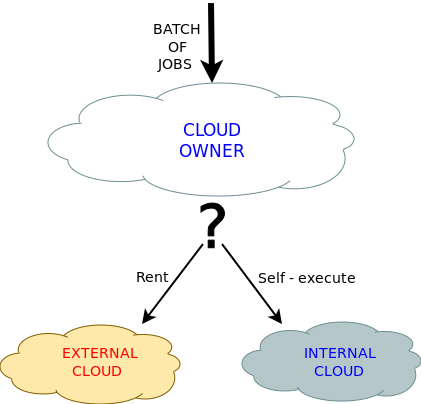
\includegraphics[width=0.48\textwidth]{Diagram1}\\[0.3cm]
For this infinite demand of the user to be met, the cloud provider has to find ways to do it without incurring any loss. One of the approaches to do it is to calculate the number of times the provider does not have the capacity to execute the load and based on that draw up an agreement with another provider to execute the load. This calculation can be predicted from past data through forecasting and by game theory (to include the current data also). The method of standard deviation can help in deciding the strategy of the cloud provider.
\section{Literature Survey}
One of the aspects of Cloud Computing is the illusion of infinite computing resources available on demand, thereby eliminating the need for Cloud Computing users to plan far ahead for provisioning. For this, realizing the economies of scale afforded by statistical multiplexing and bulk purchasing requires the construction of extremely large data-centers. Building, provisioning, and launching such a facility is a hundred-million-dollar undertaking \cite{Berkeley}.\\[0.2cm]
A system composed of a virtual network of virtual machines capable of live migration across multi-domain physical infrastructure have been constructed. By using dynamic availability of infrastructure resources and dynamic application demand, a virtual computation environment is able to automatically relocate itself across the infrastructure and scale its resources \cite{SRAS}. Thus the QoS improvements can be met using this virtual machine setup. Depending on the type of application, the generated workload can be a highly varying process that turns difficult to find an acceptable trade-off between an expensive over-provisioning able to anticipate peak loads and a sub performing resource allocation that does not mobilize enough resources. These properties can be leveraged to derive a probabilistic assumption on the mean workload of the system at different time resolutions \cite{DRMC}.\\[0.2cm]
There are many proposals that dynamically manage Virtual Machines by optimizing some objective function such as minimizing cost function, cost performance function and meeting QoS objectives. The objective function is defined as Utility property which is selected based on measures of response time, number of QoS, targets met and profit etc. \cite{SRAS}. This Utility property can then be adjusted to include factors of individual importance. They have been modified to meet needs according to current demand. But they may prove complex and  may not work in a practical virtualization cloud system with real workload. These approaches work best for stationary demands and may not give optimal solution for dynamic resource requirements. The utility property can be modified to include dynamic demands and allocation. This requires formulating the appropriate utility property that captures these demands.
\section{Design}
The process of load balancing considers factors like execution time, the number of resources required and the probability of having to wait for the resource at the server among others. Using these factors, a utility function is formulated:
\begin{center}
\setlength{\fboxrule}{0.5mm}
\fbox{$Utility =$ \large{${\frac{e}{t_{avg}} + n^{1-p} \over s}$}}\\
\end{center}
\vspace{0.1cm}
where $e$ is the execution time of the current job, $t_{avg}$ is the moving average of the execution time of all the previous jobs in the batch, $n$ is the number of resources required to execute the batch, $p$ is the waiting probability and $s$ is the batch size. Taking into account resource utilization, execution time and throughput, this function gives each of these factors a non-trivial weightage.\\[0.2cm]
The term $e \over t_{avg}$ deals with execution time and average throughput. $n^{1-p}$ deals with resource allocation. If the number of resources required is less, then the waiting probability will be less and therefore they should never become trivial, hence $n$ is raised to a factor of $1-p$.\\[0.2cm]
This function is additive because all the factors are given a non-trivial weightage whereby all of them are included in computing the utility value. In order to maintain uniformity between the batches, the batch size has been divided.\\[0.2cm]
For each batch, a forecasting method is applied with the existing utility values to compute the utility value for the next batch. The forecasting methods can depend on the trend present in these input utility data. If no trend is present, exponential smoothing can be applied and the presence of trend will shift the forecasting to Holt's Method.\\[0.2cm]
$\hspace*{3mm}/^\ast Choosing\hspace*{1mm}Forecasting\hspace*{1mm}Method^\ast/$\\
\begin{algorithmic}
\IF {$trend == true$}
	\STATE $method \gets Holt's\hspace*{1mm}Method$
\ELSE
	\STATE $method \gets Exponential\hspace*{1mm}Smoothing$ 
\ENDIF
\end{algorithmic}
\vspace{0.2cm}
The computed forecasted value is compared with the actual utility value of the batch (an average of the utility values of all the jobs in the batch) to understand the computing facilities required to execute the batch.\\[0.3cm]
$\hspace*{3mm}/^\ast Choosing\hspace*{1mm}Batch\hspace*{1mm}Strategy\hspace*{1mm}by\hspace*{1mm}Forecasting^\ast/$\\ 
\begin{algorithmic}
\IF {$forecast\hspace*{1mm}value < average\hspace*{1mm}utility$}
	\STATE $strategy \gets Rent$
\ELSE
	\STATE $strategy \gets Self-execute$
\ENDIF
\end{algorithmic}
\vspace{0.2cm}
When the value of forecast is obtained, the system prepares itself to provide computing facilities atmost equal to that of the utility value forecasted. So if the forecasted value is less than the actual utility value, then the system was not prepared to handle that load as it forecasted only lesser facilities . So the cloud owner pays rent to an external cloud who can provide the necessary computing facilities for executing the batch. If found otherwise, the cloud owner will execute the batch with the facility he owns.\\[0.2cm]
This approach only uses past information to decide the strategy even when the present data are made available. A sudden deviation in the batch load may not be captured in such a case and may result in incorrect forecasting and strategy results. So a game-theoretic approach, where the current data is also considered while deciding the strategy, is adopted.\\[0.2cm]
In this approach, two utility values are calculated for two waiting probabilities, $p_1$ and $p_2$ where $0<=p_1<=0.5$ and $0.5<p_2<=1$. The strategies of Rent and Self-execute then randomly take the $u_1$ and $u_2$ values:\\[0.3cm]
$\hspace*{3mm}/^\ast On\hspace*{1mm}Random\hspace*{1mm}Coin-toss^\ast/$\\
\begin{algorithmic}
\IF {$Coin-toss == 1$}
	\STATE $Rent \gets u_1$
	\STATE $Self-execute \gets u_2$
\ELSE
	\STATE $Self-execute \gets u_1$
	\STATE $Rent \gets u_2$
\ENDIF
\end{algorithmic}
\vspace{0.2cm}
The above random strategy can be interchanged without much effect. So, for each batch of jobs a matrix $M_{Batch Size\hspace*{0.5mm}X\hspace*{0.5mm}2}$ is created with utility values for Rent and Self-execute strategies. The maximum utility values for each strategy is then selected alongwith its corresponding rows resulting in a matrix $M'_{2\hspace*{0.5mm}X\hspace*{0.5mm} 2}$. A method of mixed strategy calculation is applied to $M'$ which chooses the strategy with the higher probability $p$.\\[0.2cm]
The strategy given by forecasting and game theory may be different. In such a case, further decision has to be taken as to which strategy should be adopted. The method of standard deviation in each conflicting batch is applied about the points:\\[0.3cm]
$\mu_1\hspace*{0.5mm}=\hspace*{0.5mm}forecasted\hspace*{1mm}value$\hspace*{3.5mm}$/^\ast Forecast\hspace*{1mm} approach^\ast/$\\
$\mu_2\hspace*{0.5mm}=\hspace*{0.5mm}equilibrium\hspace*{1mm}value$\hspace*{2mm}$/^\ast Game\hspace*{1mm}Theory\hspace*{1mm}approach^\ast/$\\[0.3cm]
Where equilibrium value is obtained as:
\begin{displaymath}
p\ast utility_p + (1-p) \ast utility_{1-p}
\end{displaymath}
The final strategy is given by the approach that has minimum standard deviation.\\[0.3cm]
$\hspace*{3mm}/^\ast In\hspace*{1mm}case\hspace*{1mm}of\hspace*{1mm}Conflict\hspace*{1mm}of\hspace*{1mm}Strategies^\ast/$
\begin{algorithmic}
\STATE $\sigma_1 \gets Standard\hspace*{1mm}Deviation\hspace*{1mm}about\hspace*{1mm}\mu_1$
\STATE $\sigma_2 \gets Standard\hspace*{1mm}Deviation\hspace*{1mm}about\hspace*{1mm}\mu_2$
\vspace{0.2cm}
\IF {$\sigma_1 < \sigma_2$}
	\STATE $strategy \gets strategy_{Forecasting}$
\ELSE
	\STATE $strategy \gets strategy_{GameTheory}$
\ENDIF
\end{algorithmic}
%\vspace{0.1cm} 
\section{Implementation}
A batch of jobs (maximum 25 jobs per batch) having randomly generated values for execution time, number of resources required and waiting probability is initially created and 1000 such batches are initialized. The first seven batches are made to randomly adopt a strategy because of the window size taken in the approach.\\[0.2cm]
The utility value for each job is calculated using the utility function and the average of these values are obtained for a batch. While applying a forecasting model, if a linear trend is observed in the average utility values for a window size of 7 consecutive batches, Holt's method is used. Otherwise exponential smoothing is used to calculate the forecast value for the next batch of jobs. A relaxation of 3 values has been provided in the forecasting model so that an almost equal distribution of Holt's and exponential model is observed. This deviation was experimentally chosen. The smoothing constants for the models were taken as $\alpha$ = 0.2 and $\beta$ = 0.1 to maintain stability of the forecast. The forecast value obtained from this approach is then used to decide the strategy using forecast by the algorithm for choosing batch strategy by forecasting.\\[0.2cm]
Further for game theory, the utility values for $p_1$ and $p_2$ probabilities are calculated for each batch and then by the selection process a $2\hspace*{0.5mm}X\hspace*{0.5mm}2$ matrix is obtained which undergoes the mixed strategy calculation. The strategy with higher probability is the strategy using game theory.\\[0.2cm]
From the above two approaches, two strategies are obtained. Whenever there is a conflict in the strategies obtained from the approaches, the strategy which gives minimum standard deviation with its respective means is finally chosen.\\[0.2cm]
For example, consider that the cloud provider receives the $i^{th}$ batch, then the forecast is done for the $(i+1)^{th}$ batch utility value which is the average of the utility values of all the jobs in the batch. If a trend is observed in these average values of $(i-7)^{th}$ batch to $i^{th}$ batch, then the forecast for the $(i+1)^{th}$ batch utility is obtained using Holt's Method; else exponential smoothing is adopted. Then when the $(i+1)^{th}$ batch is received by the provider, the average actual utility of the $(i+1)^{th}$ batch is computed and is compared with the forecasted value previously obtained. Based on the algorithm for choosing batch strategy by forecasting, either Rent or Self-execute strategy is chosen. At the same $(i+1)^{th}$ batch, two utility values are then calculated for each job in this batch using $p_1$ and $p_2$ probabilities and a matrix is constructed. The selection process is then applied to this matrix to obtain the $2\hspace*{0.5mm}X\hspace*{0.5mm}2$ matrix and finally the mixed strategy calculation is done to decide the Rent or Self-execute strategy using game theory. Thus the strategies for the $(i+1)^{th}$ batch is obtained by the two approaches. Consider a scenario whereby the Rent strategy is chosen through forecasting and Self-execute through game theory (or vice versa) for the $(i+1)^{th}$ batch, standard deviation is then applied and by the last algorithm on conflict of strategies, the final strategy to be adopted by the cloud provider is chosen for the $(i+1)^{th}$ batch.
\section{Results and Analysis}
During forecasting, the strategy adopted is seen to be biased towards the Self-execute strategy. The utility values are observed to lie within the range 1 to 10 for the values generated. So when a sudden increasing trend in the utility values is seen (observed as a greater slope), then the next forecasted value will be much higher as it takes into consideration the difference between the values while forecasting in a linear trend. This will result in the Self-execute strategy being chosen frequently. The decreasing trend phenomenon does not happen frequently as this sudden decrease cannot be seen from a high value because of the common range observed. Hence however big a decreasing trend is observed, it still lies within the acceptable range. \\[0.3cm]
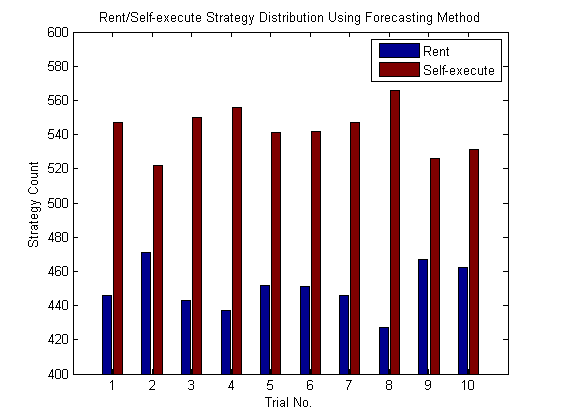
\includegraphics[width=0.49\textwidth]{forecasting1}\\[0.3cm]
An almost equal distribution of strategies of Rent and Self-execute was observed with the game theoretic approach with no strategy overpowering the other. This is because of the randomness in allocating the utility values to the strategies while constructing the matrix. This results in an unbiased evaluation of the matrix which gives an almost equal weightage to both the strategies.\\[0.3cm]
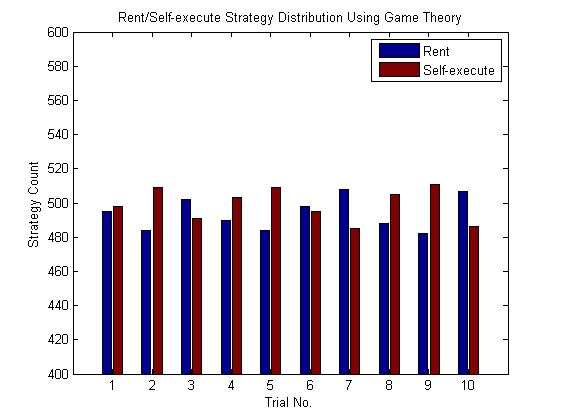
\includegraphics[width=0.49\textwidth]{Gametheory}\\[0.3cm]
The overall strategy also shows an almost equal distribution after resolving the conflicts. In case of conflicts, the final strategy obtained from the standard deviation method considers both forecasting and game theoretic approaches. In this case, the utility values of the jobs in the current batch is compared with the utility values obtained from forecasting and game theory. This method finally selects the strategy that does not deviate much from the expected value obtained from the above two approaches, thus making it easier for the cloud provider to provide the services required to execute the batch without deviating much from the services he already provides.\\[0.3cm]
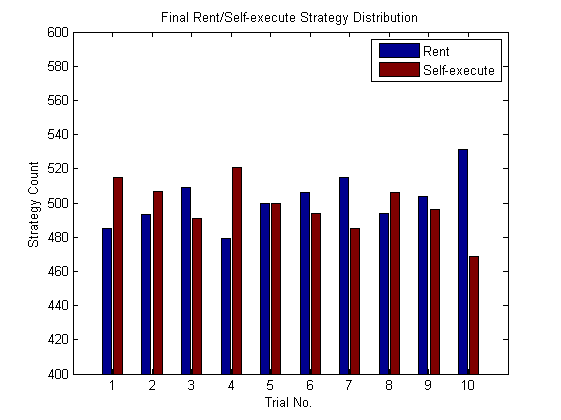
\includegraphics[width=0.5\textwidth]{final}\\[0.3cm]
The results obtained above are with respect to the randomly generated data inputs. In the real environment, certain values like waiting probability depends on factors like network congestion, efficiency of the cloud, datacenter locations, etc. So during run-time, the results obtained may vary with respect to dynamic factors. The utility function can also be further enhanced to include economic factors for the cloud provider to get a clearer picture. 
\section{Conclusion}
In this paper, we have discussed one approach of how the illusion of infinite resources in Cloud Computing can be further optimized without incurring any loss for the cloud provider. QoS can be improved and thus it provides the user with better facilities. The cloud provider can decide whether he wants to pay rent for executing the load and prevent disappointing the user or just execute only what is possible. Forecasting followed by game theory gives a better approach of including the data available till the current point and will help in correctly deciding the strategy. From these results, a cloud provider can also check the number of times he is paying rent to execute the load and based on further calculations he can decide to own more facilities such that the frequency of renting will decrease and he may earn more profit. This can be modelled as a Ski-Rental problem and further worked out.\\[0.2cm]
This paper provides one method of tackling the problem and it further opens up interesting avenues for improvement. The utility property can be changed to suit the agreement between the provider and the user. This approach considers execution time as one of the factors and this may change depending on the network traffic and other dynamic factors which will further complicate the utility property. There can be different utility functions that can be used considering more parameters. Other game-theoretic concepts and forecasting models can also be used to obtain the results. Since the avenues are deep and the domain is still growing, updates on this problem will keep on increasing until an optimal solution is reached.
\begin{thebibliography}{1}

\bibitem{NIST} Mell, Peter, and Timothy Grance. ``The NIST definition of Cloud Computing (draft)." \emph{NIST special publication} 800 (2011): 145.

\bibitem{QOS} Armstrong, Django, and Karim Djemame. ``Towards Quality of Service in the Cloud." In \emph{Proc. of the 25th UK Performance Engineering Workshop.} 2009.

\bibitem{RAD} Endo, Patricia Takako, Andre Vitor de Almeida Palhares, Nadilma Nunes Pereira, Glauco Estacio Goncalves, Djamel Sadok, Judith Kelner, Bob Melander, and J. Mangs. ``Resource allocation for distributed cloud: concepts and research challenges." \emph{Network, IEEE} 25, no. 4 (2011): 42-46.

\bibitem{Berkeley} Armbrust, Michael and Fox, Armando and Griffith, Rean and Joseph, Anthony D. and Katz, Randy H. and Konwinski, Andrew and Lee, Gunho and Patterson, David A. and Rabkin, Ariel and Stoica, Ion and Zaharia, Matei. ``Above the Clouds: A Berkeley View of Cloud Computing." \emph{Technical report}, no. UCB/EECS-2009-28 (2009).

\bibitem{SRAS} Vinothina Sr, V. ``A Survey on Resource Allocation Strategies in Cloud Computing." \emph{International Journal} (2012).

\bibitem{DRMC} Goncalves, Paulo, R. O. Y. Shubhabrata, Thomas Begin, and Patrick Loiseau. ``Dynamic Resource Management in Clouds: A Probabilistic Approach." \emph{IEICE Transactions on Communications} 95, no. 8 (2012): 2522-2529.

\bibitem{Book} Han, Zhu, Dusit Niyato, Walid Saad, Tamer Başar, and Are Hjørungnes. \emph{Game theory in wireless and communication networks: theory, models, and applications.} Cambridge University Press, 2011.

\bibitem{TimeSeries} Kalekar, Prajakta S. ``Time series forecasting using Holt-Winters exponential smoothing." \emph{Kanwal Rekhi School of Information Technology} (2004).

\bibitem{Wiki1} Ski Rental problem,\ \url{http://en.wikipedia.org/wiki/Ski_rental_problem}.

\bibitem{Wiki2} Standard Deviation,\ \url{http://en.wikipedia.org/wiki/Standard_deviation}.

\bibitem{Wiki3} Forecasting Method,\ \url{http://nptel.iitm.ac.in/courses/110106045}.

\bibitem{SAS} SAS Products and Solution Documentation.

\end{thebibliography}


% that's all folks
\end{document}


